% Drawing 86/01-8 -- folder 86, batch 01, archive page 7 (PDF page 8).
% Transcription: en bas, (B$_2$) : une construction en perspective de l'icosaèdre — la moitié avant du solide, sommets $a$, $c'$, $b'$, $w$, $v$, $b$, $u$, $c$, $a'$, prise dans un réseau de longues droites qui concourent en trois points de fuite (deux en haut, à gauche et à droite, un en bas) ; à gauche, un triangle hachuré, pointe en bas.
% Kind: perspective construction of the icosahedron with vanishing lines; hatched triangle. Method 2 (schematic redraw from the facsimile). Status: partial.
% Notes: Drawn: the nine named vertices and the edges between them that the page shows (c'-a, a-b', c'-w, a-w, a-v, w-v, v-b', c'-b, w-b, w-u, v-u, v-c, b'-c, b-u, u-c, b-a', c-a', and u-a' dashed), with their letters; the three vanishing points and the three long lines joining them (in ink on the page, like the rest); the hatched triangle at the left with the horizontal stroke across it. Left out: the other construction lines, some twenty long strokes from the vanishing points through the vertices and beyond, which cross one another over the whole figure and could not be assigned one by one; the circled label (B_2) is given at the lower left. Still differs: which vertices each construction line passes through is not established, so the perspective construction itself is not reproduced, only its frame; the hatching of the small triangle was a pattern over the whole triangle (redrawn on 2026-11-14, below). Decided by a machine pass, 2026-11-12: the two inner vertices of the upper row are read w (left) and v (right) and the middle one of the lower row u, as on (B_1). Not checked by a reader. Overlaid on the 400 dpi colour crop on 2026-11-12: every vertex, label and the frame lie within 1 mm of the page; the three long lines of the frame were in the pencil style, but they are in the same blue ink as the figure, and are now drawn plain. Redrawn 2026-11-12 (issue 128): to check again. Overlay check 2026-11-13 (issue 147, Claude claude-opus-5-5): the redraw, rasterised by the skill's previewer (not compiled: no TeX in the session), laid over the 300 dpi colour crop of the scan (250 ppi). The frame of three long lines, the icosahedron, its letters and the hatched triangle lie on their ink to within about 1 unit. Still differs, as said above: the many construction lines of the perspective are not reproduced, only the frame, and the hatching covered the whole small triangle (redrawn on 2026-11-14). 2026-11-14, Claude Opus 5.5, issue 147 second pass: the hatching of the small triangle redrawn stroke by stroke from the 400 dpi colour scan on a gridded crop at 36 pixels per unit: it is a zigzag of eleven blue strokes, most of them above the horizontal stroke, two running below it towards the lower vertex; the horizontal stroke follows its slight bend. Overlay with the local TikZ interpreter (not compiled: no TeX in the session): the drawn strokes lie on their ink to within about one unit. Still differs: where the zigzag is densest, between the middle of the horizontal stroke and the right side, two or three of its strokes run together and are not all separated; the construction lines of the perspective are not reproduced, only the frame.
% Coordinates: 1 unit = 1 mm = 1/100 of the crop width (bbox in page fractions: [0.28, 0.47, 0.92, 0.8]).
% Redrawn by Claude (claude-fable-5-2), issue #128, 2026-11-12; not checked by a human; not compiled (no TeX in the session).
% Revised by Claude (claude-opus-5-5) 2026-11-12 (issue #128, overlay check on the 400 dpi colour facsimile): vertices, labels and the frame confirmed within 1 mm; the three long lines of the frame, in ink on the page, no longer drawn in the pencil style. Not compiled. Status: partial.
% Checked by Claude (claude-opus-5-5) 2026-11-13 (issue #147): overlaid on the 300 dpi colour facsimile; not compiled (no TeX in the session). Status: partial.
% Rights: reproduces part of the work -- behind RENDER_TRANSCRIPTS, never published by itself.
\documentclass[tikz,border=3pt]{standalone}
\usepackage{amsmath,amssymb}
\usetikzlibrary{patterns,arrows.meta}
\tikzset{pencil/.style={black!45}, struck/.style={black!35}, mpt/.style={circle,draw,inner sep=1.3pt}, pt/.style={circle,fill,inner sep=0.9pt}, opt/.style={circle,draw,fill=white,inner sep=1.1pt}}
\begin{document}
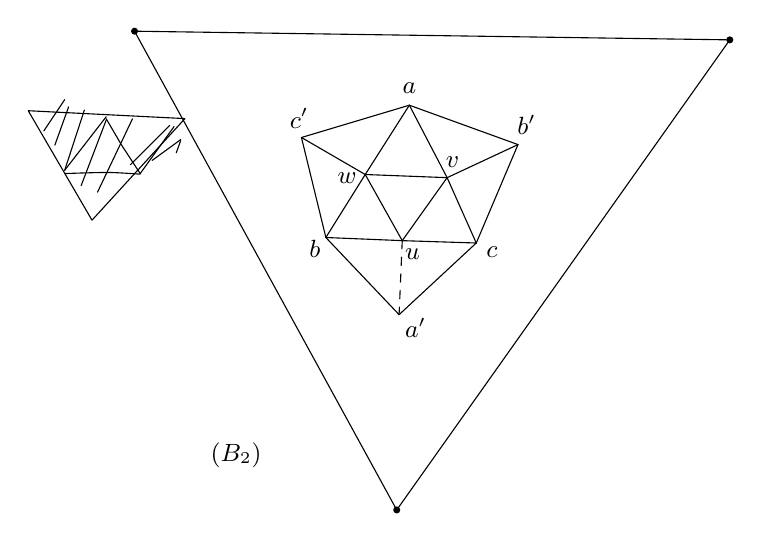
\begin{tikzpicture}[x=1mm,y=1mm,line cap=round,line join=round,font=\scriptsize]
\draw (38.4,-22.2) -- (52.1,-18.1);
\draw (52.1,-18.1) -- (65.9,-23.1);
\draw (38.4,-22.2) -- (46.5,-26.9);
\draw (52.1,-18.1) -- (46.5,-26.9);
\draw (52.1,-18.1) -- (56.9,-27.3);
\draw (46.5,-26.9) -- (56.9,-27.3);
\draw (56.9,-27.3) -- (65.9,-23.1);
\draw (38.4,-22.2) -- (41.5,-34.9);
\draw (46.5,-26.9) -- (41.5,-34.9);
\draw (46.5,-26.9) -- (51.2,-35.3);
\draw (56.9,-27.3) -- (51.2,-35.3);
\draw (56.9,-27.3) -- (60.6,-35.6);
\draw (65.9,-23.1) -- (60.6,-35.6);
\draw (41.5,-34.9) -- (51.2,-35.3);
\draw (51.2,-35.3) -- (60.6,-35.6);
\draw (41.5,-34.9) -- (50.8,-44.7);
\draw (60.6,-35.6) -- (50.8,-44.7);
\draw[dashed] (51.2,-35.3) -- (50.8,-44.7);
\draw (17.2,-8.7) -- (92.8,-9.8);
\draw (17.2,-8.7) -- (50.5,-69.5);
\draw (92.8,-9.8) -- (50.5,-69.5);
\node[pt] at (17.2,-8.7) {};
\node[pt] at (92.8,-9.8) {};
\node[pt] at (50.5,-69.5) {};
\draw (3.7,-18.8) -- (23.6,-19.8) -- (11.8,-32.7) -- cycle;
% the hatching: his zigzag strokes, each as on the page
\draw (5.69,-21.36) -- (8.33,-17.39);
\draw (7.08,-23.17) -- (8.83,-18.31);
\draw (8.33,-26.36) -- (10.83,-18.72);
\draw (8.33,-26.36) -- (13.61,-19.56);
\draw (10.42,-28.31) -- (13.61,-19.97);
\draw (12.50,-29.14) -- (16.94,-19.83);
\draw (13.61,-19.83) -- (15.56,-23.17) -- (17.92,-26.78);
\draw (16.67,-25.67) -- (21.67,-20.67);
\draw (17.92,-26.78) -- (22.22,-20.81);
\draw (19.44,-25.11) -- (23.06,-22.47);
\draw (22.50,-24.14) -- (23.06,-22.61);
\draw plot[smooth, tension=0.5] coordinates {(8.33,-26.78) (13.89,-26.64) (17.92,-26.86)};
\node[inner sep=1pt] at (52.1,-15.9) {\small $a$};
\node[inner sep=1pt] at (38.1,-19.8) {\small $c'$};
\node[inner sep=1pt] at (67,-20.6) {\small $b'$};
\node[inner sep=1pt] at (44.2,-27.3) {\small $w$};
\node[inner sep=1pt] at (57.6,-25.3) {\small $v$};
\node[inner sep=1pt] at (40.1,-36.3) {\small $b$};
\node[inner sep=1pt] at (52.5,-37) {\small $u$};
\node[inner sep=1pt] at (62.6,-36.7) {\small $c$};
\node[inner sep=1pt] at (52.9,-46.4) {\small $a'$};
\node[inner sep=1pt] at (30.1,-62.5) {\small $(B_2)$};
\end{tikzpicture}
\end{document}
